\documentclass{acm_proc_article-sp}



\begin{document}


\title{Search engine for {\ttlit Politics} Lovers}

% AUTHORS
\numberofauthors{2} 
\author{
\alignauthor
David Dias\titlenote{Master Student}\\
       \affaddr{IST, Technical University of Lisbon}\\
       \affaddr{Av. Prof. Doutor Aníbal Cavaco Silva}\\
       \affaddr{2744-016 Porto Salvo, Portugal}\\
       \email{david.dias@ist.utl.pt}
% 2nd. author
\alignauthor
Rui Francisco\titlenote{Master Student}\\
       \affaddr{Institute for Clarity in Documentation}\\
       \affaddr{Av. Prof. Doutor Aníbal Cavaco Silva}\\
       \affaddr{2744-016 Porto Salvo, Portugal}\\
       \email{rui.miguel.guerreiro.francisco@ist.utl.pt}
}
\maketitle
\begin{abstract}
This project was developed in the Data Mining Course of the Communication Networks Master in Engineering, the goal is to develop a robust and reliable search engine and data crawler for information related with politics and their participants. It was development mechanisms of evaluating popularity and relationships as well as a quick search engine for quality results
\end{abstract}

\keywords{TD-IDF, BM25, Search, Crawler, Politics, Personalities, Data-Mining, Big Data, Feeds, News, Sentiment, Natural Language Processing} % NOT required for Proceedings


\section{Introduction}
Super Search Engine is a Political news crawler, analyser and indexer that enables it's users to find with excellent performance and result quality news related with political personalities, know their popularity and understand how this personalities relate to each other. This document describes the implementation realised , the challenges, the algorithms, the design decisions and the results achieved by the authors of the system.

In the following parts of the documents, the architecture will be described as well as the data collecting and searching mechanisms, how each individual component is built and finally the conclusions achieved by building a search engine about a category of news.


\section{Arquitecture}
\textit{Super Search Engine} Architecture is divided in modules loosely coupled, they are interchangeable as long they respect the \textit{I/O} expected, the goal with this type of implementation is enabling enhancing each individual component without breaking the system in itself. There is a module for collection news, one for entity extraction, news search, sentiment analysis, do the search and one extra to measure the results. All data produced/collected is saved in collections of a \textit{MongoDB} instance and indexed in \textit{Whoosh}. In Figure 1 we can see the overview of the architecture, section 2.1 and 2.2 will explain the Mining and Searching Scheme respectively and each component will be introduced with proper reasoning in the algorithm choice

	\begin{figure}[h]
   	\centering
   	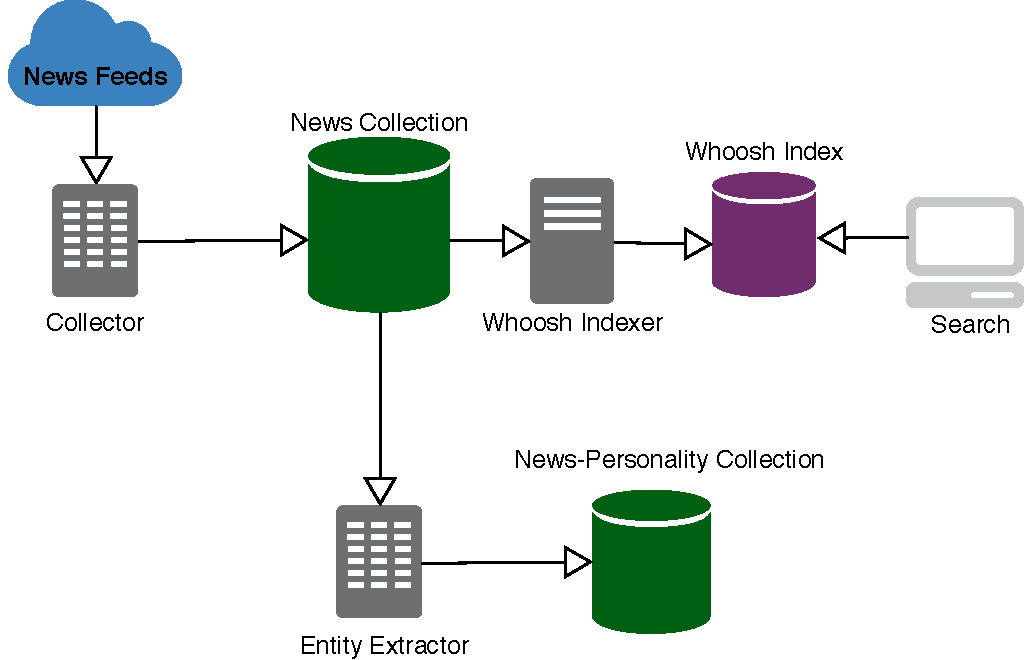
\includegraphics[width=0.45\textwidth]{architecture.png}
   	\caption{Super Search Architecture}
	\end{figure}


\subsection{Mining scheme}

Our Data-Mining scheme is composed by 4 different operations done asynchronously to offer operation interchangeability, the sequence is done as follows:

\begin{enumerate}
  \item Collect the news using a feedparser plus a content collector 
  \item Index the news in Whoosh by Title and Body so they are both searchable
  \item Extract the entities found in each news if they are political personalities
  \item Analyse the sentiment present in each news collected and attribute it to the personality present
\end{enumerate} 

When this process is finished, we've enough information prepared for our Searching Scheme, described in section 2.2. The Mining Scheme is described in Figure 2.

We use \textit{MongoDB} which is a \textit{Document Oriented Database} for the data store for it's developer friendly functionality and fast data indexing, Super Search Engine takes advantage of \textit{MongoDB}, for example in upserts (update, if not exists, insert), saving time in news comparisons and verifications, it's scalability led us also to very quick deployment since it's schema less.
We use \textit{Whoosh} for indexing our data collection for easy sorting of documents base on \textit{BM25} and \textit{TF-IDF}, giving strong measurements of relevance for documents in function of a query.

	\begin{figure}[h]
   	\centering
   	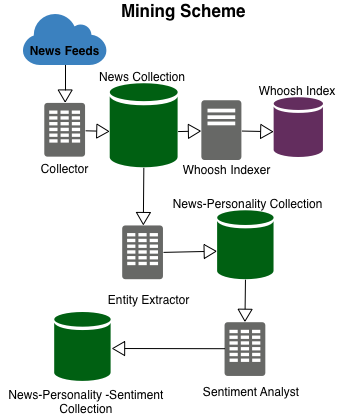
\includegraphics[width=0.40\textwidth]{MiningScheme.png}
   	\caption{Data Mining Scheme of Super Search Engine}
	\end{figure}


\subsection{Searching scheme}

Our Search Scheme was developed on top of all the data we collected, matching different signals to have best results in our search. We can see how it progresses in Figure 3.

	\begin{figure}[h]
   	\centering
   	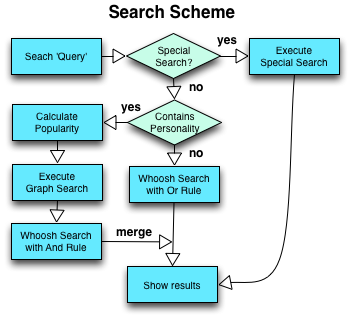
\includegraphics[width=0.40\textwidth]{SearchScheme.png}
   	\caption{Seach Scheme of Super Search Engine}
	\end{figure}

After receiving a query, the first question comes if it is a Special Search, which can be:

\begin{itemize}
  \item "Who is more popular" - Returns which is the person most popular
  \item "Who is more hated" - Returns which person is less popular 
\end{itemize}

If one of this options is selected, it is showed immediately the answer to the user.

The next step is seeing if the query introduced by the user contains a Personality, this is one of the key ingredients of super search, if in fact the query has a Personality we will execute the following operations

\begin{enumerate}
  \item Calculate the popularity of the personality (or personalities in the query), regarding the data set available, giving details of how many news that person shows. By popularity we mean the accumulated sentiment from all the news that person appears. 
  \item Execute a "graph search", a graph search is calculating how strong is the relation between the searched personality and the others in the data set, the more times they appear together, the stronger is the relation
  \item Search in whoosh index with "And Rule", what we mean by this is that if a personality name is "Miguel Francisco" we are going to look for news when that both names appear together and not alone, since Miguel and Francisco are both common names.
\end{enumerate} 

With this we are going to merge this results with a "Or Rule", so we can also find the news that relate to the rest of the query and find the best match possible, so we can create the best results.

\subsection{Components}

Instead of doing a massive, monolithic application, Super Search is divided into 5 individual interchangeable components, so it's easy to enhance the results by tuning each part individually, if I/O for each of them is respected.

\subsubsection{NewsCollection and Storage}

For collecting the news we use feedparser and Beautiful Soup Modules for python, this is a systematic and sequential process, after each feed is fetched(in "newsCollector/collector.py") with feedparser, we make a fetch of the Article ID of the post using Beautiful Soup(in "newsCollector/contentCollector.py"), so we can get the full news content, creating the information that will fuel our search more rich.

\subsubsection{News Search}
 
News Search is implemented in the folder "NewsSearch" but it's divided into 2 phases, the first one dedicated to indexing for the Data-Mining Scheme, implemented in the file "indexInWhoosh.py", the second phase is under "NewsSearch.py", "BM25" and "TFIDF", the last two give us a search on the Whoosh index using BM25 and TFIDF respectively, using equal weights for both algorithms. The "NewsSearch.py" makes an API available for Searching using "OR Rule" or "AND Rule" and mixing two searches to be used by Super Search

\subsubsection{Extraction of Personalities}

Extraction of Personalities is done on the "entityExtraction" Module, the purpose of this Module is only to identify which of the names are present in each news and then compare it with our list of political names to see if it's a match, to make this happen we use Natural Language Processing (made available by the nltk module) to find which names are words in first hand. The process follows the algorithm:

\begin{enumerate}
  \item Analyse next news in news collection at the MongoDB instance
  \item Tokenize with each sentence with "nltk.sent\_tokenize"
  \item Classify each word with "nltk.pos\_tag"
  \item Creates chunks using the chunker function for name entity nltk.ne\_chunck
  \item Verify each PERSON node to see if match to our list of political personalities, if yes, then we consider that news has some comment on that personallity and insert it on the NewsPersonality Collection on the MongoDB instance
\end{enumerate} 

\subsubsection{Sentiment Analysis}

Our implementation of our Sentiment Analysis procedure is on "sentimentAnalysis/sentimentFlex.py", to achieve best results, we used an library of words associated with the sentiment they transmitted called SentiLex\cite{sent}. 

To make it easy to find the sentiment in each sentence, the implemented a routine called "polarity" which will receive the news, break it down by sentences and then evaluate it accordingly, in the end we will sum the value of all words that have polarity associated with. With this calculation we managed to find out if the sentiment present in a news is positive or negative.

\subsubsection{Super Search}

SuperSearch is implemented in the folder "SuperSearch", here is where all the dots connect to efficient searches with all the information retrieved in the components showed before.
SuperSearch performs 3 types of searches, for personalities, special search and, or for news.

When is perform a search to know what is the most or less popular personality the functions that are performs are whoIsMorePopular and whoIsMoreHated. These two functions are only executed when a search is made with the following words: “who is more popular” or “who is more hated”.The functions receive a data structure that contains the name of the personalities and its popularity. This data structure is created by the function orderedByPopularity that build a data structure with the personalities names and their popularity. And orders this structure using this function sorded python.

If the query contains personalities, we identify those personalities to perform a graphSearch (in graphSearch.py) to display the relations between personalities in news, this means we can know how many times a personality X appears in same news as personality Y. Next we look into popularity (in popularity.py) to discover how the personalities searched are rated, this is handled by the function personalityPopularity, which will look into all the news in the database and see how this personality rates in each one of them to sum every value and discover the total popularity .

Finally we will search for the news related to the query, this depends on the type of research done. If the research have a name of personality, the results will be a merge of two searches, one to find all the news with that personality name and the second one with all the query, this is to make sure that if we search for a personality we prioritise the news related to that person. If there was no personality in the query from the begining the only step shown is the display of the news, these are presented by order of relevance based in the SUM of BM25 and TFIDF metrics of each news. 



\section{Result analysis}
To test our implementation, we executed two kinds of analysis, one based in the traditional measures, Precision, Recall and F1 metrics, and a more human testing approach, the second approach is less unfeasible for large data sets and real world live production services, however, due to our data-set being dynamic and growing only at a small rate, it was impossible for us to classify relevant documents for high amount of queries to execute the tests automatically.

We are not going to reference the results from measures Precision, Recall and F1 metrics, since the results were artificial and not demonstrative due to small amount of documents and available sets of query->relevant document, making us unable to create the confidence interval for those, however the implementation to execute them sits on the "precisionRecallFone" folder of our project

From our Human testing approach our results were extremely positive, all searches for Personalities retrieved all the news containing that personality.

\section{Future Work}
For this project the time was very limited, with more time we can increase a lot our results, specially in real world conditions, with datasets big enough to cause lot's of noise and confusion, our next approach will be implementing a nltk trainer which will be able to understand portuguese dialect to detect which sentiment is attached to who and not attribute to the all sentence the same sentiment.

Another feature we want to implement is using d3.js for data visualisation, the original graph idea was designed to have relation graphs between personalities and see the connection between parties, events and other interesting facts, that could help the user better understand what is happening in the politics world.

\section{Conclusions}

You can only achieve great results in a search engine with big datasets, the results able to retrieve from a small amount of data aren't enough to estimate the true behaviour in real world environments, where the confusion and entropy among the results is high.

Precision, Recall and F1 metrics are good measures for quality of results, however they are biased with our perception of reality, by judging our datasets in those metrics, we have to know prior to classification which documents we consider best or worse and that is based on pure human judgement, getting this datasets of relevant documents for each query is not easy cause the perception of each human is also biased by the environment, culture and life experiences that he has been put up through. This is why we see a tendency for ad agencies and search engines to start classifying by "one size fit's all metrics" but yet tailor each set of results based on the user past experiences , this algorithms have seen a greater increase of efficiency since the generalisation of social networks, where there has been a great input of information about each person profile to the searching algorithms.

Natural Language Processing is as well as powerful as it is expensive, getting it tune to the right tone, the right word, the right sentence for every language, adding also the culture aspects into it can be an work expensive work, however, the power the recognise patterns that help us to understand what the user wants or what the user meant leads us to better and more solid results in our searches.

In conclusion this projects was super interesting in a way of understanding the concepts behind data mining and data-search, however it could benefit greatly if the timeline was extended (starting sooner and ending later) creating checkpoints for data mining, data processing and data visualisation, creating more feedback cycles it's possible to understand if the right path if followed.

\bibliographystyle{ieeetr}
\bibliography{bibliografia}


\end{document}
